\begin{table*}[t]
\centering
\caption{Per-seed supervised MM-UAV transfer metrics. Each final checkpoint was evaluated once on the frozen exposed devval split.}
\label{tab:mmuav-transfer-seeds}
\scriptsize
\setlength{\tabcolsep}{3.4pt}
\begin{tabular}{@{}rlrrrrrr@{}}
\toprule
Seed & Method & AP & AP50 & AP75 & AR1 & AR10 & AR100\\
\midrule
0 & Scratch Equal & 0.2270 & 0.5628 & 0.1416 & 0.1765 & 0.3366 & 0.3536\\
0 & TriAir Init Equal & 0.2155 & 0.5512 & 0.1281 & 0.1682 & 0.3271 & 0.3445\\
0 & TriAir Init Reliability & 0.2118 & 0.5384 & 0.1205 & 0.1662 & 0.3190 & 0.3384\\
\addlinespace
1 & Scratch Equal & 0.2150 & 0.5448 & 0.1218 & 0.1662 & 0.3258 & 0.3422\\
1 & TriAir Init Equal & 0.2192 & 0.5539 & 0.1274 & 0.1672 & 0.3234 & 0.3393\\
1 & TriAir Init Reliability & 0.2082 & 0.5390 & 0.1173 & 0.1641 & 0.3215 & 0.3382\\
\addlinespace
2 & Scratch Equal & 0.2283 & 0.5632 & 0.1386 & 0.1772 & 0.3415 & 0.3580\\
2 & TriAir Init Equal & 0.2186 & 0.5527 & 0.1208 & 0.1692 & 0.3271 & 0.3471\\
2 & TriAir Init Reliability & 0.2253 & 0.5580 & 0.1384 & 0.1709 & 0.3326 & 0.3498\\
\bottomrule
\end{tabular}
\end{table*}

\begin{table*}[t]
\centering
\caption{Paired AP differences for the frozen MM-UAV transfer benchmark. Values are descriptive; no significance test is claimed.}
\label{tab:mmuav-paired-ap}
\scriptsize
\setlength{\tabcolsep}{3.2pt}
\begin{tabular}{@{}lrrrr@{}}
\toprule
Comparison & Seed 0 & Seed 1 & Seed 2 & Mean $\pm$ SD\\
\midrule
Init Equal $-$ Scratch & -0.0115 & +0.0042 & -0.0097 & $-0.0056\pm0.0086$\\
Init Reliability $-$ Init Equal & -0.0036 & -0.0111 & +0.0067 & $-0.0027\pm0.0089$\\
Init Reliability $-$ Scratch & -0.0152 & -0.0068 & -0.0030 & $-0.0083\pm0.0062$\\
\bottomrule
\end{tabular}
\end{table*}

\paragraph{Seed-level evidence boundary.}
The seed-level records reproduce the frozen three-seed means and sample standard deviations in \tabref{tab:mmuav-transfer}. Source initialization does not improve AP consistently under equal fusion, and the reliability-aware initialized variant is below the from-scratch control for all three AP pairs. The results are reported descriptively on an exposed devval split and are not treated as statistical-significance or independent-generalization evidence.

\begin{figure*}[t]
\centering
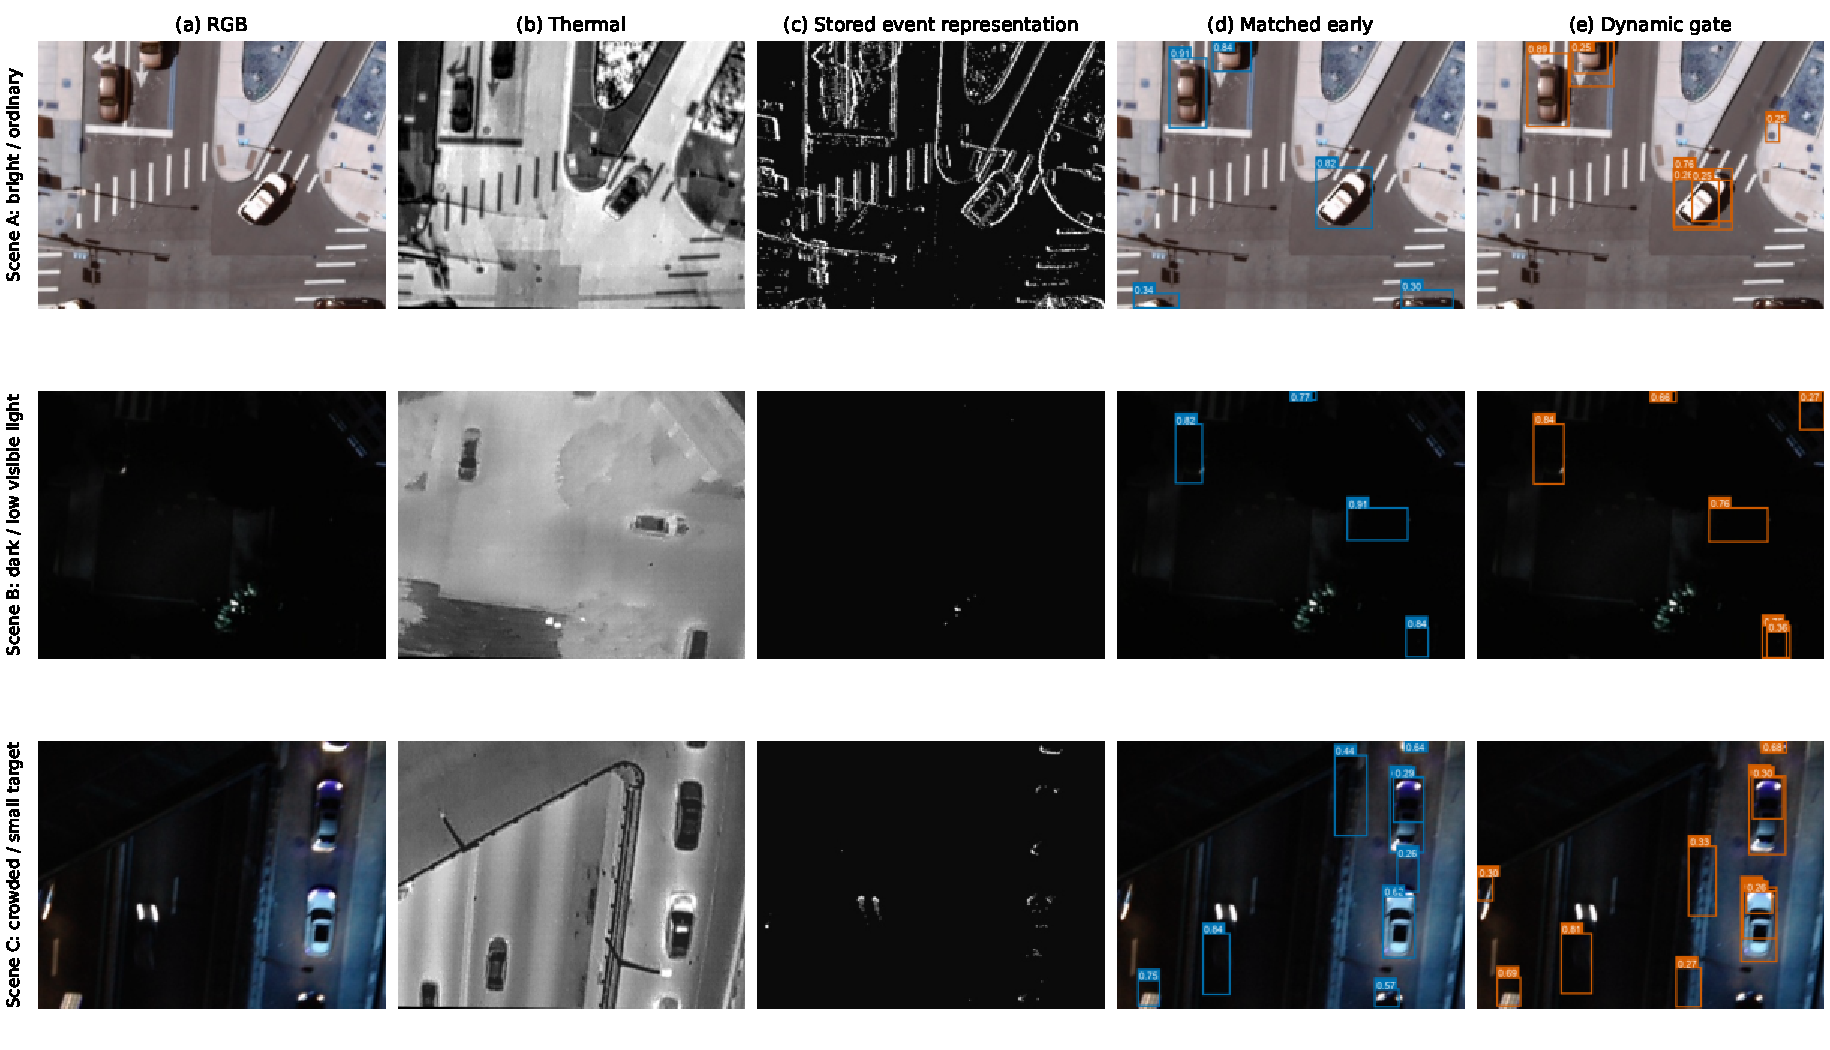
\includegraphics[width=0.99\textwidth]{figures/fig6_real_qualitative.pdf}
\caption{Qualitative detections on deterministically selected TriAir component-disjoint development-validation samples. Columns show the RGB observation, thermal channel, stored event representation, matched early-fusion predictions, and dynamic-gate predictions from fixed seed-0 checkpoints. Samples are selected from predeclared image descriptors rather than model performance. Bounding boxes and confidence scores are direct checkpoint outputs under one fixed display threshold; no manual box editing is applied.}
\label{fig:real-qualitative}
\end{figure*}

Figure~\ref{fig:real-qualitative} is illustrative rather than quantitative. The three samples come from distinct validation components under the frozen model-independent selection rule, and both prediction columns use score threshold 0.25, NMS IoU 0.60, and at most 100 detections. The panels do not establish external generalization, calibrated reliability, or physical sensor-failure robustness.

\section{Discussion and Limitations}
\subsection{In-Domain Dynamic Fusion and Event Contribution}
The three-seed component-disjoint results and completed causal controls support a mechanism-level conclusion for nominal input: RA-RepDet gate/no-dropout exceeds matched early fusion, fixed equal stems, and learned deterministic projection, and it remains positive against all three controls under component-macro bootstrap. Modality dropout has a small negative full-input main effect and lowers nominal AP inside the gated architecture. It is therefore an optional robustness regularizer rather than the defining mechanism or nominal default.

The V81 and V86 experiments clarify the role of the event stream. Event-only is the weakest standalone modality at $0.1949\pm0.0012$ AP, whereas thermal-only reaches $0.5196\pm0.0196$ and RGB-only reaches $0.4473\pm0.0033$. Nevertheless, in the matched dynamic-gating comparison, adding event to RGB+thermal increases mean AP from $0.6912\pm0.0280$ to $0.7251\pm0.0121$, AP75 from $0.8409\pm0.0241$ to $0.8742\pm0.0081$, and AR100 from $0.7673\pm0.0232$ to $0.7917\pm0.0098$, while AP50 remains nearly unchanged. The AP gain is positive in two of three seeds and negative in seed 0. The defensible conclusion is therefore complementary event contribution on average under the frozen development protocol, not uniform per-seed improvement or statistical significance.

The matched channel-removal factorial analysis provides a separate robustness result. Gate/no-dropout is fragile to event removal, while gate-plus-dropout is robust; the event-removal dropout main effect and gate-by-dropout interaction are large. Robustness to zeroed channels is therefore mainly associated with dropout training in this condition. Controlled blur and attenuation further show that gate weights are not monotonic sensor-quality indicators. The weights are task-driven fusion coefficients, and channel removal does not emulate sensor drift, asynchronous failure, spatial misregistration, field-of-view change, or other physical failure modes.

\subsection{Alignment Dominates Direct Cross-Sensor Transfer}
The MM-UAV experiments provide a complementary boundary on the TriAir result. The zero-shot model executes correctly and emits finite boxes for every target image, but the boxes do not align with the target annotations under an independently normalized, physically unregistered five-channel adapter. Reliability weights cannot correct geometry that is inconsistent before meaningful feature correspondence is established. The near-zero zero-shot result therefore should not be interpreted as evidence that the detector is numerically unstable or that reliability-aware fusion is intrinsically ineffective; it isolates a severe adapter and acquisition-domain mismatch.

Learned target-domain feature alignment and supervision restore AP from effectively zero under the frozen naive-grid stress test to $0.2234\pm0.0073$ for the matched from-scratch equal-fusion model. This large recovery shows that a compatible target representation and geometry contract is a prerequisite in this cross-sensor setting. Once that requirement is met, the differences among initialization and fusion variants are comparatively small and do not favor the source-initialized variants on average.

\subsection{Negative Transfer under High Parameter Coverage}
Approximately 99.20\% of destination parameter and buffer elements are initialized from exact name-and-shape-compatible TriAir tensors in both initialized transfer variants; this is not a sample match rate or architecture-identity claim. Despite the high transfer coverage, TriAir Init Equal reaches $0.2178\pm0.0020$ AP and TriAir Init Reliability reaches $0.2151\pm0.0090$, both below the $0.2234\pm0.0073$ from-scratch control. The paired mean AP differences are $-0.0056$ for initialized equal fusion versus scratch, $-0.0027$ for initialized reliability versus initialized equal fusion, and $-0.0083$ for initialized reliability versus scratch. This is a documented negative-transfer outcome under one frozen 10-epoch protocol, not evidence that tensor copying failed.

The experiment does not prove that every transfer strategy would fail. Layer-wise learning rates, partial reinitialization, progressive unfreezing, longer schedules, or explicit source-target representation matching were not tested. Because the devval split was exposed during engineering and target-domain labels are used, the correct conclusion is limited to this supervised transfer benchmark rather than general cross-dataset superiority or failure.

\subsection{Evaluation Scope}
The component-disjoint split protocol is deliberately stronger than an exact-duplicate check, but it has a defined scope. It enforces component disjointness for the locked graph composed of exact RGB content, perceptual-hash candidates, and human-adjudicated adjacent-or-near-identical observations. It cannot demonstrate that all possible scene correlations are absent. Numeric filename identifiers were not treated as verified temporal metadata. The guard partition is a locked internal holdout, not an independently acquired public test set.

The causal and primary TriAir development evidence remains validation-only because the component-disjoint validation partition participates in within-run checkpoint retention. The guard evidence is stronger because it is evaluated after checkpoint lock, but it comes from the same local dataset inventory. The MM-UAV zero-shot experiment is performed on a previously exposed devval split with a deliberately naive unregistered adapter, while the supervised benchmark uses MM-UAV training labels. A separately acquired and sealed sensor-compatible test set would be required for independent external-generalization claims.

V84 did not reuse the 837-image internal holdout. A same-protocol published comparison was also not produced. The pinned official TriModalDet implementation uses its own random 80/20 split, excludes empty-label samples, and lacks the frozen evaluator and checkpoint-selection interface. Replacing those contracts would constitute a substantial new adaptation rather than a direct reproduction, so no cross-protocol published number is reported.

\section{Conclusion}
RA-RepDet is the sample-dependent dynamic-gate model, with gate/no-dropout as its primary nominal-accuracy variant. It reaches $0.7251\pm0.0121$ AP on component-disjoint TriAir development-validation and exceeds matched early, fixed-equal, and deterministic-projection controls under both seed summaries and component-macro bootstrap. Modality dropout is not responsible for the nominal gain, but it is important for robustness to deterministic channel removal, especially event removal.

Checkpoint-backed single-modality and matched event-contribution experiments refine the multimodal interpretation. Thermal is the strongest standalone stream and event-only is the weakest, yet adding event to the matched RGB+thermal dynamic system yields a descriptive mean gain of $+0.0339$ AP, $+0.0333$ AP75, and $+0.0244$ AR100, with positive AP gains in two of three seeds and virtually unchanged AP50. Event information is therefore complementary on average in this protocol, but the evidence does not support uniform or statistically significant improvement.

The cross-dataset analysis further limits the scope of the method claim. Frozen unregistered transfer to MM-UAV fails, supervised feature alignment restores useful performance, and high-coverage TriAir initialization does not improve the three-seed mean over the target-only control. Taken together, the evidence supports lightweight task-driven dynamic fusion under a leakage-aware TriAir development protocol while emphasizing that cross-sensor transfer requires explicit alignment and may exhibit negative transfer. We do not claim calibrated physical sensor reliability, statistical significance, same-protocol superiority over a published comparator, or independent external generalization.

\section*{Statements and Declarations}
\bmhead{Funding}
This research received no specific grant from any funding agency in the public, commercial, or not-for-profit sectors.

\bmhead{Competing Interests}
The authors declare that they have no competing interests.

\bmhead{Author Contributions}
Nan Xin: Conceptualization, methodology, software, validation, formal analysis, investigation, data curation, visualization, and writing--original draft. Xueting Jin: Supervision, project administration, resources, methodology, and writing--review and editing. Both authors reviewed and approved the manuscript.

\bmhead{Data Availability}
TriAir and MM-UAV are publicly available research datasets and should be obtained from their original public providers under the applicable access and use terms. This repository does not redistribute raw sensor data, annotations, transformed derivatives, or trained weights. The project records frozen manifests, split and audit reports, evaluator settings, checkpoint hashes for all nine V81 single-modality replications, training traces, and compact result artifacts sufficient to identify the experimental subsets and protocols. The MM-UAV experiments use an exposed devval split and are not official untouched-test performance.

\bmhead{Code Availability}
The project repository contains the model implementation, frozen manifests, split and audit utilities, standardized evaluators, MM-UAV transfer scripts, checkpoint identity records, raw standardized evaluator JSON files, and compact result artifacts used in this manuscript. Raw sensor arrays, label archives, trained weights, and transient prediction caches are not included.

\sloppy
\begin{thebibliography}{99}
\bibitem{zhao2019object} Zhao, Z.-Q., Zheng, P., Xu, S.-T., Wu, X.: Object detection with deep learning: A review. IEEE Trans. Neural Netw. Learn. Syst. 30(11), 3212--3232 (2019). \url{https://doi.org/10.1109/TNNLS.2018.2876865}
\bibitem{cheng2016survey} Cheng, G., Han, J.: A survey on object detection in optical remote sensing images. ISPRS J. Photogramm. Remote Sens. 117, 11--28 (2016). \url{https://doi.org/10.1016/j.isprsjprs.2016.03.014}
\bibitem{xia2022dota} Xia, G.-S. et al.: DOTA: A large-scale dataset for object detection in aerial images. IEEE Trans. Pattern Anal. Mach. Intell. 44(10), 5969--5988 (2022). \url{https://doi.org/10.1109/TPAMI.2021.3074724}
\bibitem{zhu2017deepRS} Zhu, X.X. et al.: Deep learning in remote sensing: A comprehensive review and list of resources. IEEE Geosci. Remote Sens. Mag. 5(4), 8--36 (2017). \url{https://doi.org/10.1109/MGRS.2017.2762307}
\bibitem{baltrusaitis2019multimodal} Baltru\v{s}aitis, T., Ahuja, C., Morency, L.-P.: Multimodal machine learning: A survey and taxonomy. IEEE Trans. Pattern Anal. Mach. Intell. 41(2), 423--443 (2019). \url{https://doi.org/10.1109/TPAMI.2018.2798607}
\bibitem{gallego2022event} Gallego, G. et al.: Event-based vision: A survey. IEEE Trans. Pattern Anal. Mach. Intell. 44(1), 154--180 (2022). \url{https://doi.org/10.1109/TPAMI.2020.3008413}
\bibitem{kapoor2023leakage} Kapoor, S., Narayanan, A.: Leakage and the reproducibility crisis in machine-learning-based science. Patterns 4(9), 100804 (2023). \url{https://doi.org/10.1016/j.patter.2023.100804}
\bibitem{cawley2010overfitting} Cawley, G.C., Talbot, N.L.C.: On over-fitting in model selection and subsequent selection bias in performance evaluation. J. Mach. Learn. Res. 11, 2079--2107 (2010)
\bibitem{wang2024repvit} Wang, A., Chen, H., Lin, Z., Han, J., Ding, G.: RepViT: Revisiting mobile CNN from ViT perspective. In: Proc. IEEE/CVF Conf. Comput. Vis. Pattern Recognit., pp. 15909--15920 (2024)
\bibitem{lin2017fpn} Lin, T.-Y. et al.: Feature pyramid networks for object detection. In: Proc. IEEE Conf. Comput. Vis. Pattern Recognit., pp. 2117--2125 (2017). \url{https://doi.org/10.1109/CVPR.2017.106}
\bibitem{tian2019fcos} Tian, Z., Shen, C., Chen, H., He, T.: FCOS: Fully convolutional one-stage object detection. In: Proc. IEEE/CVF Int. Conf. Comput. Vis., pp. 9627--9636 (2019). \url{https://doi.org/10.1109/ICCV.2019.00972}
\bibitem{ren2017faster} Ren, S., He, K., Girshick, R., Sun, J.: Faster R-CNN: Towards real-time object detection with region proposal networks. IEEE Trans. Pattern Anal. Mach. Intell. 39(6), 1137--1149 (2017). \url{https://doi.org/10.1109/TPAMI.2016.2577031}
\bibitem{lin2020focal} Lin, T.-Y., Goyal, P., Girshick, R., He, K., Doll\'{a}r, P.: Focal loss for dense object detection. IEEE Trans. Pattern Anal. Mach. Intell. 42(2), 318--327 (2020). \url{https://doi.org/10.1109/TPAMI.2018.2858826}
\bibitem{ramachandram2017deep} Ramachandram, D., Taylor, G.W.: Deep multimodal learning: A survey on recent advances and trends. IEEE Signal Process. Mag. 34(6), 96--108 (2017). \url{https://doi.org/10.1109/MSP.2017.2738401}
\bibitem{li2017pixel} Li, S., Kang, X., Fang, L., Hu, J., Yin, H.: Pixel-level image fusion: A survey of the state of the art. Inf. Fusion 33, 100--112 (2017). \url{https://doi.org/10.1016/j.inffus.2016.05.004}
\bibitem{ma2019surveyfusion} Ma, J., Ma, Y., Li, C.: Infrared and visible image fusion methods and applications: A survey. Inf. Fusion 45, 153--178 (2019). \url{https://doi.org/10.1016/j.inffus.2018.02.004}
\bibitem{li2019densefuse} Li, H., Wu, X.-J.: DenseFuse: A fusion approach to infrared and visible images. IEEE Trans. Image Process. 28(5), 2614--2623 (2019). \url{https://doi.org/10.1109/TIP.2018.2887342}
\bibitem{lichtsteiner2008sensor} Lichtsteiner, P., Posch, C., Delbr\"uck, T.: A 128$\times$128 120 dB 15 $\mu$s latency asynchronous temporal contrast vision sensor. IEEE J. Solid-State Circuits 43(2), 566--576 (2008). \url{https://doi.org/10.1109/JSSC.2007.914337}
\bibitem{gehrig2021dsec} Gehrig, M., Aarents, W., Gehrig, D., Scaramuzza, D.: DSEC: A stereo event camera dataset for driving scenarios. IEEE Robot. Autom. Lett. 6(3), 4947--4954 (2021). \url{https://doi.org/10.1109/LRA.2021.3068942}
\bibitem{neverova2016moddrop} Neverova, N., Wolf, C., Taylor, G.W., Nebout, F.: ModDrop: Adaptive multi-modal gesture recognition. IEEE Trans. Pattern Anal. Mach. Intell. 38(8), 1692--1706 (2016). \url{https://doi.org/10.1109/TPAMI.2015.2461544}
\bibitem{pan2010transfer} Pan, S.J., Yang, Q.: A survey on transfer learning. IEEE Trans. Knowl. Data Eng. 22(10), 1345--1359 (2010). \url{https://doi.org/10.1109/TKDE.2009.191}
\bibitem{yosinski2014transfer} Yosinski, J., Clune, J., Bengio, Y., Lipson, H.: How transferable are features in deep neural networks? In: Advances in Neural Information Processing Systems 27, pp. 3320--3328 (2014)
\bibitem{iaboni2026trimodal} Iaboni, C., Abichandani, P.: Tri-Modal Fusion Transformers for UAV-based Object Detection. In: Proc. IEEE/CVF Conf. Comput. Vis. Pattern Recognit., pp. 4373--4382 (2026)
\bibitem{xu2025mmuav} Xu, T., Gu, J., Zhu, X.-F., Wu, X.-J., Kittler, J.: A Tri-Modal Dataset and a Baseline System for Tracking Unmanned Aerial Vehicles. arXiv:2511.18344 (2025)
\end{thebibliography}
\end{document}
